% Created 2018-09-18 mar 14:01
% Intended LaTeX compiler: pdflatex
\documentclass[xcolor={usenames,svgnames,dvipsnames}]{beamer}
\usepackage[utf8]{inputenc}
\usepackage[T1]{fontenc}
\usepackage{graphicx}
\usepackage{grffile}
\usepackage{longtable}
\usepackage{wrapfig}
\usepackage{rotating}
\usepackage[normalem]{ulem}
\usepackage{amsmath}
\usepackage{textcomp}
\usepackage{amssymb}
\usepackage{capt-of}
\usepackage{hyperref}
\usepackage{color}
\usepackage{listings}
\usepackage{mathpazo}
\usepackage{gensymb}
\usepackage{amsmath}
\usepackage{esdiff}
\bibliographystyle{plain}
\AtBeginSubsection[]{\begin{frame}[plain]\tableofcontents[currentsubsection,sectionstyle=show/shaded,subsectionstyle=show/shaded/hide]\end{frame}}
\AtBeginSection[]{\begin{frame}[plain]\tableofcontents[currentsection,hideallsubsections]\end{frame}}
\usepackage[emulate=units]{siunitx}
\sisetup{fraction=nice, decimalsymbol=comma, retain-unity-mantissa = false}
\newunit{\wattpeak}{Wp}
\newunit{\watthour}{Wh}
\newunit{\amperehour}{Ah}
\hypersetup{colorlinks=true, linkcolor=Blue, urlcolor=Blue}
\renewcommand{\thefootnote}{\fnsymbol{footnote}}
\beamertemplatenavigationsymbolsempty
\setbeamertemplate{footline}[frame number]
\setbeamercolor{alerted text}{fg=blue!50!black} \setbeamerfont{alerted text}{series=\bfseries}
\usetheme[hideothersubsections]{Goettingen}
\usecolortheme{rose}
\usefonttheme{serif}
\author{Oscar Perpiñán Lamigueiro}
\date{Septiembre 2018}
\title{Análisis Clásico de Circuitos de Segundo Orden}
\subtitle{Teoría de Circuitos III}
\hypersetup{
 pdfauthor={Oscar Perpiñán Lamigueiro},
 pdftitle={Análisis Clásico de Circuitos de Segundo Orden},
 pdfkeywords={},
 pdfsubject={},
 pdfcreator={Emacs 25.2.2 (Org mode 9.1.13)}, 
 pdflang={Spanish}}
\begin{document}

\maketitle

\section{Introducción}
\label{sec:org2345c92}

\begin{frame}[label={sec:org421ecc1}]{Circuitos de Segundo Orden}
\begin{itemize}
\item Circuitos que tienen \alert{dos elementos de acumulación} que intercambian energía, y parte resistiva que disipa energía.
\item \alert{Ecuación diferencial de segundo orden}: la respuesta natural incluye exponenciales decrecientes y quizás señal sinusoidal.
\item Circuitos típicos:
\begin{itemize}
\item RLC serie
\item RLC paralelo
\end{itemize}
\end{itemize}
\end{frame}
\begin{frame}[label={sec:orgc496cf5}]{Respuesta natural y forzada}
\begin{itemize}
\item El método de resolución analiza el circuito en dos etapas:
\begin{itemize}
\item Sin fuentes: \alert{respuesta natural} (la energía acumulada en \(t < 0\) se redistribuye).
\item Con fuentes: \alert{respuesta forzada} (determinada por la forma de onda de las fuentes).
\end{itemize}
\end{itemize}
\end{frame}

\section{Circuito RLC serie}
\label{sec:org63bc792}
\begin{frame}[label={sec:org4c902c1}]{Circuito básico}
\begin{center}
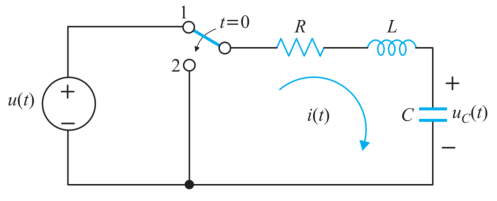
\includegraphics[width=.9\linewidth]{figs/RLC_serie.pdf}
\end{center}

\[
  Ri(t) + L\diff{i(t)}{t} + \frac{1}{C}\int_{-\infty}^t i(t') \mathrm{d}t' = 0
\]
\end{frame}

\begin{frame}[label={sec:org8fe12ec}]{Ecuación diferencial (respuesta natural)}
\begin{center}
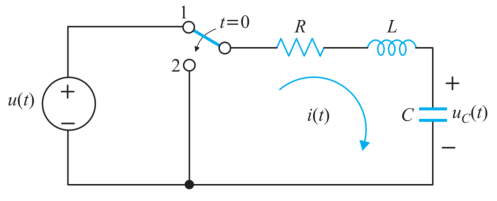
\includegraphics[width=.9\linewidth]{figs/RLC_serie.pdf}
\end{center}

\begin{align*}
  L\diff[2]{i}{t} + R\diff{i}{t} + \frac{1}{C} i &= 0\\
  \diff[2]{i}{t} + \frac{R}{L} \diff{i}{t} + \frac{1}{LC} i &= 0\\
\end{align*}
\end{frame}

\begin{frame}[label={sec:orgb27d37d}]{Solución}
\begin{block}{Ecuación característica}
\[
s^2 + \frac{R}{L} s + \frac{1}{LC} = 0  
\]
\end{block}

\begin{block}{Solución}
\[
  s_{1,2} = -\frac{R}{2L} \pm \sqrt{\left(\frac{R}{2L}\right)^2 - \frac{1}{LC}}
\]
\end{block}
\end{frame}


\begin{frame}[label={sec:org34626aa}]{Solución con parámetros}
\begin{block}{Ecuación característica}
\begin{columns}
\begin{column}{.5\columnwidth}
\[
s^2 + 2\alpha s + \omega_0^2 = 0  
\]
\end{column}
\begin{column}{.5\columnwidth}
\begin{align*}
  \alpha &= \frac{R}{2L}\\
  \omega_0 &= \frac{1}{\sqrt{LC}}\\
  \xi &= \frac{\alpha}{\omega_0}
\end{align*}
\end{column}
\end{columns}
\end{block}

\begin{block}{Solución}
\[
  s_{1,2} = -\alpha \pm \sqrt{\alpha^2 - \omega_0^2}
\]

\[
  i_n(t) = A_1 e^{s_1 t} + A_2 e^{s_2 t}
\]
\end{block}
\end{frame}

\begin{frame}[label={sec:orge896e08}]{Posibles soluciones}
\begin{block}{\(\alpha > \omega\), \(\xi > 1\)}
\begin{itemize}
\item \(s_{1,2}\): dos soluciones reales (negativas) distintas
\item Circuito \alert{sobreamortiguado}.
\end{itemize}
\end{block}

\begin{block}{\(\alpha = \omega\), \(\xi = 1\)}
\begin{itemize}
\item \(s_{1,2}\): solución real doble.
\item Circuito con \alert{amortiguamiento crítico}.
\end{itemize}
\end{block}

\begin{block}{\(\alpha < \omega\), \(\xi < 1\)}
\begin{itemize}
\item \(s_{1,2}\): dos soluciones complejas conjugadas
\item Circuito \alert{subamortiguado}.
\end{itemize}
\end{block}
\end{frame}

\begin{frame}[label={sec:org3d81218}]{Tipos de Respuesta}
\begin{itemize}
\item Tipo de respuesta determinado por relación entre \(R\) y \(L\), \(C\) (disipación y almacenamiento).
\item Resistencia crítica (\(\alpha = \omega_0\), \(\xi = 1\)):
\end{itemize}

\[
  R_{cr} = 2\sqrt{\frac{L}{C}}
\]

\begin{block}{Tipos}
\begin{itemize}
\item \(R > R_{cr}\), \(\alpha > \omega\), \(\xi > 1\): \alert{sobreamortiguado}
\item \(R = R_{cr}\),  \(\alpha = \omega\), \(\xi = 1\): \alert{amortiguamiento crítico}
\item \(R < R_{cr}\),  \(\alpha < \omega\), \(\xi < 1\): \alert{subamortiguado}
\end{itemize}
\end{block}
\end{frame}

\begin{frame}[label={sec:org013dcec}]{Circuito Sobreamortiguado (\(\alpha > \omega_0\))}
\[
  i_n(t) = A_1 e^{s_1 t} + A_2 e^{s_2 t}
\]

\begin{center}
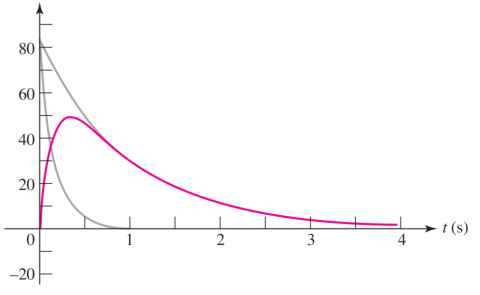
\includegraphics[width=.9\linewidth]{figs/Sobreamortiguado_HKD.pdf}
\end{center}
\end{frame}

\begin{frame}[label={sec:orgf5d9b6e}]{Amortiguamiento Crítico (\(\alpha = \omega_0\))}
\[
  i_n(t) = (A_1 + A_2 t) e^{s t} 
\]

\begin{center}
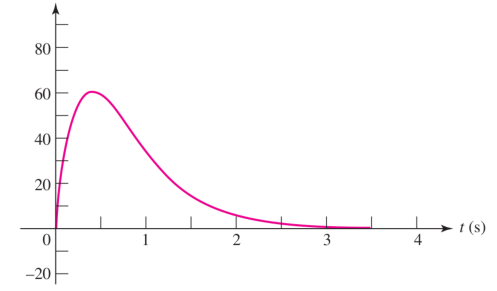
\includegraphics[width=.9\linewidth]{figs/AmortiguamientoCritico_HKD.pdf}
\end{center}
\end{frame}


\begin{frame}[label={sec:orgb804b73}]{Circuito Subamortiguado (\(\alpha < \omega\))}
\[
  i_n(t) = (B_1\cos(\omega_d t) + B_2\sin(\omega_d t)) e^{-\alpha t}
\]

\begin{center}
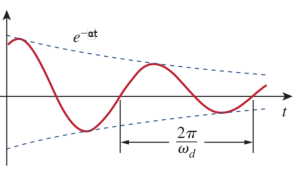
\includegraphics[width=.9\linewidth]{figs/Subamortiguado_AS.pdf}
\end{center}

\[
\omega_d = \sqrt{\omega_0^2 - \alpha^2}
\]
\end{frame}

\begin{frame}[label={sec:orgbb4ced6}]{Comparación}
\begin{center}
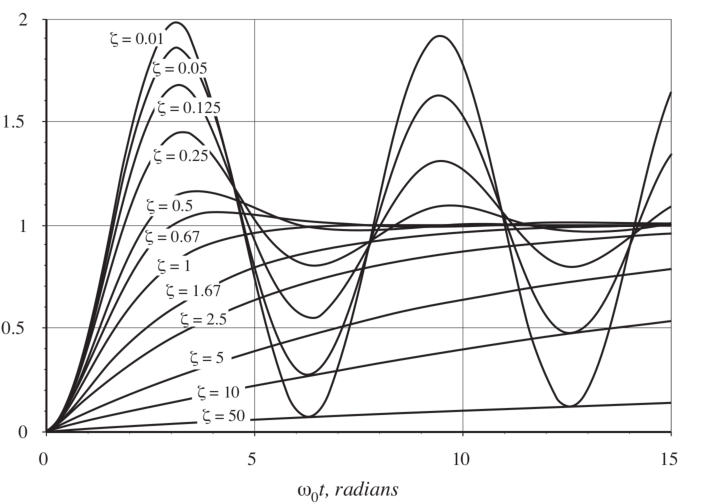
\includegraphics[width=.9\linewidth]{figs/DampingRatio.pdf}
\end{center}
\end{frame}

\begin{frame}[label={sec:orge16b534}]{Valores Importantes}
\begin{center}
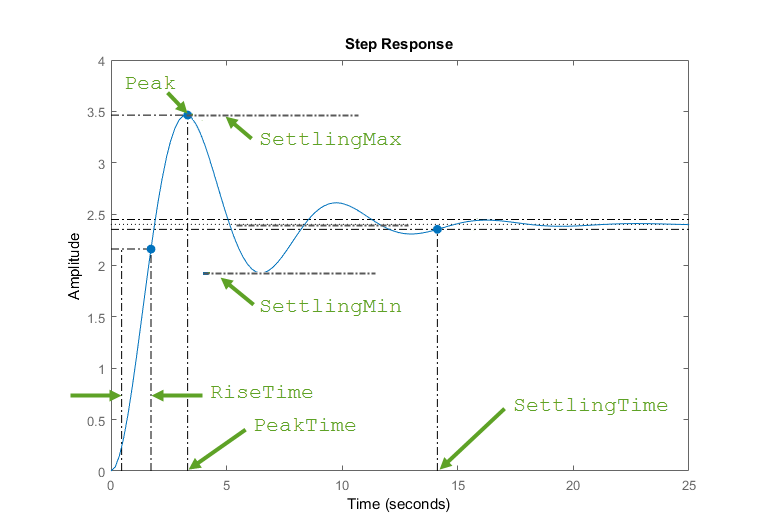
\includegraphics[width=.9\linewidth]{figs/RespuestaEscalon_SegundoOrden.png}
\end{center}
\end{frame}

\begin{frame}[label={sec:orgaa8dcee}]{Valores Importantes}
\begin{itemize}
\item \alert{Tiempo de Subida}: tiempo para subir de 10\% al 90\% del valor en régimen permanente.

\item \alert{Tiempo de Establecimiento}: tiempo para que la diferencia entre la respuesta y el régimen permanente permanezca dentro de una banda del 1\%.

\item \alert{Valor máximo} y \alert{Tiempo del Valor Máximo}.

\item \alert{Sobretensión} o \alert{Sobrecorriente}: porcentaje del valor máximo respecto del régimen permanente.
\end{itemize}
\end{frame}

\section{Circuito RLC paralelo}
\label{sec:org000e9ae}
\begin{frame}[label={sec:org2b12d18}]{Circuito básico}
\begin{center}
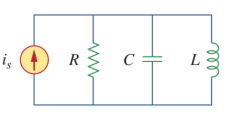
\includegraphics[width=.9\linewidth]{figs/RLC_paralelo.pdf}
\end{center}

\[
  Gu(t) + C\diff{u(t)}{t} + \frac{1}{L}\int_{-\infty}^t u(t') \mathrm{d}t' = i_s(t)
\]
\end{frame}

\begin{frame}[label={sec:org1cb91d6}]{Ecuación diferencial (respuesta natural)}
\begin{center}
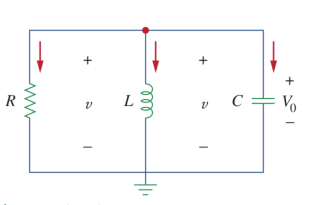
\includegraphics[width=.9\linewidth]{figs/RLC_paralelo0.pdf}
\end{center}

\[
  \diff[2]{u}{t} + \frac{G}{C} \diff{u}{t} + \frac{1}{LC} u = 0
\]
\end{frame}

\begin{frame}[label={sec:org9788531}]{Solución}
\begin{block}{Ecuación característica}
\[
s^2 + \frac{G}{C} s + \frac{1}{LC} = 0  
\]
\end{block}

\begin{block}{Solución}
\[
  s_{1,2} = -\frac{G}{2C} \pm \sqrt{\left(\frac{G}{2C}\right)^2 - \frac{1}{LC}}
\]
\end{block}
\end{frame}


\begin{frame}[label={sec:org9914205}]{Solución con parámetros}
\begin{block}{Ecuación característica}
\begin{columns}
\begin{column}{.5\columnwidth}
\[
s^2 + 2\alpha s + \omega_0^2 = 0  
\]
\end{column}
\begin{column}{.5\columnwidth}
\begin{align*}
  \alpha &= \frac{G}{2C}\\
  \omega_0 &= \frac{1}{\sqrt{LC}}\\
  \xi &= \frac{\alpha}{\omega_0}
\end{align*}
\end{column}
\end{columns}
\end{block}

\begin{block}{Solución}
\[
  s_{1,2} = -\alpha \pm \sqrt{\alpha^2 - \omega_0^2}
\]

\[
  u_n(t) = A_1 e^{s_1 t} + A_2 e^{s_2 t}
\]
\end{block}
\end{frame}



\begin{frame}[label={sec:org23510ea}]{Tipos de Respuesta}
\begin{itemize}
\item Tipo de respuesta determinado por relación entre \(G\) y \(L\), \(C\) (disipación y almacenamiento).
\item Conductancia crítica (\(\alpha = \omega_0\), \(\xi = 1\)):
\end{itemize}

\[
  G_{cr} = 2\sqrt{\frac{C}{L}}
\]

\begin{block}{Tipos}
\begin{itemize}
\item \(G > G_{cr}\), \(\alpha > \omega\), \(\xi > 1\): \alert{sobreamortiguado}
\item \(G = G_{cr}\),  \(\alpha = \omega\), \(\xi = 1\): \alert{amortiguamiento crítico}
\item \(G < G_{cr}\),  \(\alpha < \omega\), \(\xi < 1\): \alert{subamortiguado}
\end{itemize}
\end{block}
\end{frame}

\begin{frame}[label={sec:org5c8ba92}]{Tipos de Respuesta}
\begin{itemize}
\item Circuito Sobreamortiguado (\(\alpha > \omega_0\))
\end{itemize}
\[
  u_n(t) = A_1 e^{s_1 t} + A_2 e^{s_2 t}
\]
\begin{itemize}
\item Amortiguamiento Crítico (\(\alpha = \omega_0\))
\end{itemize}
\[
  u_n(t) = (A_1 + A_2 t) e^{s t} 
\]

\begin{itemize}
\item Circuito Subamortiguado (\(\alpha < \omega\))
\end{itemize}
\[
  u_n(t) = (B_1\cos(\omega_d t) + B_2\sin(\omega_d t)) e^{-\alpha t}
\]
\end{frame}


\section{Respuesta Completa}
\label{sec:org8d7320e}
\begin{frame}[label={sec:org6c70bc2}]{Condiciones Iniciales}
\begin{block}{Dos constantes a determinar}
Son necesarias dos tipos de condiciones iniciales:

\begin{columns}
\begin{column}{.5\columnwidth}
\begin{align*}
  u_C(0^+) &= u_C(0^-)\\
  \diff*{u_c}{t}{t = 0^+} &= \frac{1}{C} i_C(0^+)\\
\end{align*}
\end{column}

\begin{column}{.5\columnwidth}
\begin{align*}
  i_L(0^+) &= i_L(0^-)\\
  \diff*{i_L}{t}{t = 0^+} &= \frac{1}{L}u_L(0^+)\\
\end{align*}
\end{column}
\end{columns}
\end{block}

\begin{block}{Derivadas en el origen}
Para obtener valores de las derivadas en el origen hay que resolver el circuito en \(t = 0^+\) empleando las condiciones de continuidad.
\end{block}
\end{frame}

\begin{frame}[label={sec:org520f9a0}]{Circuitos Equivalentes}
\begin{center}
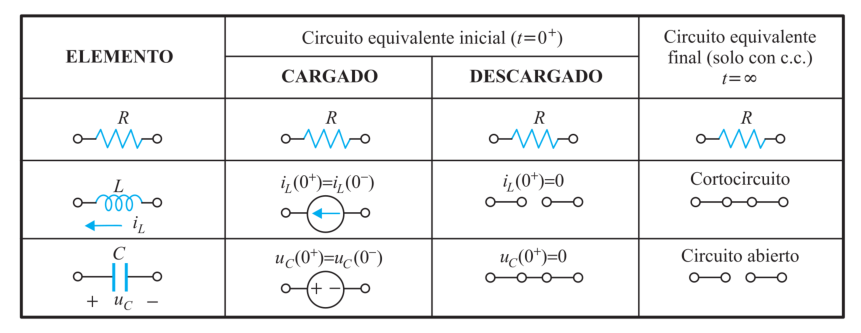
\includegraphics[width=.9\linewidth]{figs/CondicionesIniciales_CircuitosEquivalentes.pdf}
\end{center}
\begin{itemize}
\item Sustituir fuentes de tensión \(u_g(t)\) por \(u_g(0^+)\).
\item Sustituir fuentes de corriente \(i_g(t)\) por \(i_g(0^+)\).
\item Sustituir bobinas por fuentes de corriente \(i_L(0^+)\).
\item Sustituir condensadores por fuentes de tensión \(u_C(0^+)\).
\item Calcular tensiones y corrientes en circuito.
\end{itemize}
\end{frame}

\begin{frame}[label={sec:org0c31e5d}]{Derivadas en \(t = 0^+\): ejemplo RLC serie}
\begin{center}
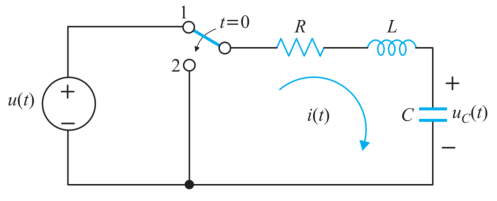
\includegraphics[width=.9\linewidth]{figs/RLC_serie.pdf}
\end{center}

\begin{align*}
  \diff*{i_L}{t}{t = 0^+} &= \frac{1}{L} u_L(0^+) = - \frac{1}{L}\left(R i_L(0^+) + u_c(0^+)\right)\\
  u_L(0^+) &= -u_R(0^+) - u_c(0^+)\\
  u_R(0^+) &= R i_L(0^+)
\end{align*}
\end{frame}

\begin{frame}[label={sec:org4b9c15e}]{Derivadas en \(t = 0^+\): ejemplo RLC paralelo}
\begin{center}
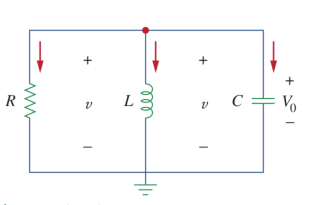
\includegraphics[height=0.5\textheight]{figs/RLC_paralelo0.pdf}
\end{center}

\begin{align*}
  \diff*{u_c}{t}{t = 0^+} &= \frac{1}{C}i_C(0^+) = - \frac{1}{C} \left( \frac{1}{R} u_C(0^+) +  i_L(0^+)\right)\\
  i_C(0^+) &= -i_R(0^+) - i_L(0^+)\\
  i_R(0^+) &= \frac{1}{R} u_C(0^+)
\end{align*}
\end{frame}


\begin{frame}[label={sec:org633d955}]{Respuesta Completa}
Las condiciones iniciales deben evaluarse teniendo en cuenta la respuesta forzada (si existe).
\begin{align*}
  f(0^+) &= f_n(0^+) + f_{\infty}(0^+)\\
  \diff*{f}{t}{t = 0^+} &= \diff*{f_n}{t}{t = 0^+} + \diff*{f_{\infty}}{t}{t = 0^+}  
\end{align*}
\end{frame}

\begin{frame}[label={sec:orge3b7ad2}]{Ejemplo}
Circuito RLC paralelo sobreamortiguado con generador de corriente DC funcionando en \(t > 0\). 

\begin{block}{Respuesta Completa}
\[
  u_c(t) = U_{\infty} + A_1 e^{s_1 t} + A_2 e^{s_2 t}
\]
\end{block}

\begin{block}{Condiciones Iniciales}
\begin{align*}
u_c(0^+) &= U_\infty + A_1 + A_2\\
\diff*{u_C}{t}{t = 0^+} &= 0 + A_1 s_1 + A_2 s_2
\end{align*}
\end{block}
\end{frame}


\section{Ejercicios Recomendados}
\label{sec:org344abc5}

\begin{frame}[label={sec:orgc84541e}]{Ejercicios}
\begin{itemize}
\item AS: Ejemplos 8.5, 8.7, 8.8 y 8.9
\item HKD: Ejemplos 9.3, 9.7, 9.8, y 9.9 + 9.10
\item FM: Ejemplos de aplicación 4.9 y 4.10
\end{itemize}
\end{frame}
\end{document}